\section{\textit{Proxy Re-Encryption} (PRE)}

\textit{Proxy Re-Encryption} (PRE) adalah varian dari skema enkripsi kunci publik (\textit{public-key encryption}) yang dirancang untuk mendelegasikan hak akses dekripsi.
PRE memungkinkan penerima untuk mendekripsi data tanpa perlu identitas kriptografi privat milik penerima.
Dalam skema ini, sebuah entitas \textit{semi-trusted proxy} diberikan kemampuan untuk mengubah sebuah \textit{ciphertext} yang awalnya dienkripsi menggunakan kunci publik pengguna pertama (\textit{Delegator}), menjadi \textit{ciphertext} baru yang dapat didekripsi menggunakan kunci privat pengguna kedua (\textit{Delegatee}) \parencite{nunez2017proxy}. 
Ilustrasi cara kerja PRE dapat dilihat pada Gambar~\ref{fig:mekanisme-pre}.

\begin{figure}[htbp]
	\centering
	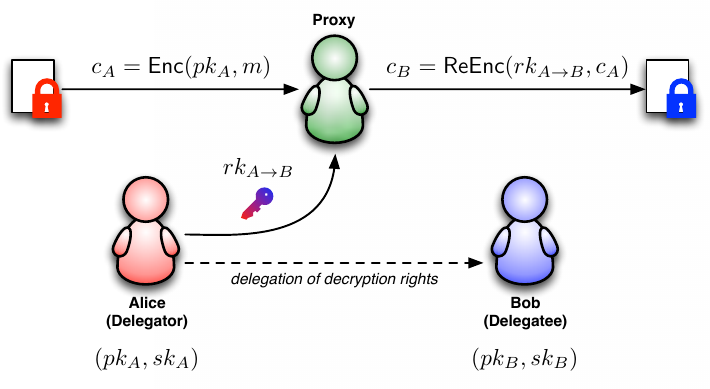
\includegraphics[width=\textwidth]{resources/chapter-2/mekanisme_pre.png}
	\caption{Mekanisme \textit{Proxy Reencryption} \parencite{nunez2017proxy}}\label{fig:mekanisme-pre}
\end{figure}

Secara formal, sebuah skema PRE standar direpresentasikan oleh sekumpulan fungsi algoritmik (\textsf{KeyGen}, \textsf{ReKeyGen}, \textsf{Enc}, \textsf{ReEnc}, \textsf{Dec}) \parencite{nunez2017proxy}:

\begin{enumerate}
    \item $\mathsf{KeyGen}(1^\kappa) \rightarrow (pk, sk)$: Algoritme pembentukan kunci yang menerima parameter keamanan $\kappa$ dan menghasilkan pasangan kunci publik ($pk$) dan kunci privat ($sk$) untuk pengguna.
    \item $\mathsf{Enc}(pk_A, m) \rightarrow C_A$: Algoritme enkripsi yang mengenkripsi pesan $m$ menggunakan kunci publik Delegator ($pk_A$) untuk menghasilkan \textit{ciphertext} awal $C_A$.
    \item $\mathsf{ReKeyGen}(sk_A, pk_B, (sk_B)) \rightarrow rk_{A \to B}$: Algoritme pembuatan token delegasi. Delegator menggunakan kunci privatnya ($sk_A$) dan representasi kunci \textit{Delegatee} (seperti $pk_B$ atau $sk_B$ tergantung skema) untuk menghasilkan \textit{Re-Encryption Key} ($rk_{A \to B}$). Kunci inilah yang dikirim ke proxy.
    \item $\mathsf{ReEnc}(rk_{A \to B}, C_A) \rightarrow C_B$: Algoritme transformasi buta. Proxy menggunakan token $rk_{A \to B}$ untuk mengubah $C_A$ menjadi \textit{ciphertext} baru $C_B$.
    \item $\mathsf{Dec}(sk_B, C_B) \rightarrow m$: Algoritme dekripsi. \textit{Delegatee} menggunakan kunci privatnya sendiri ($sk_B$) untuk mengekstraksi pesan $m$ dari $C_B$.
\end{enumerate}

% Untuk memahami bagaimana PRE mengubah data tanpa membuka lapisannya, kita meninjau skema PRE pertama yang diajukan oleh Blaze, Bleumer, dan Strauss (BBS98), yang dibangun di atas struktur aljabar enkripsi ElGamal \parencite{nunez2017proxy, ateniese2006improved}.

% Sistem beroperasi pada sebuah grup siklik $\mathbb{G}$ berorde prima $q$ dengan generator $g$.
% \begin{itemize}
%     \item \textbf{Kunci Pengguna:} Alice (Delegator) memiliki $sk_A = a \in \mathbb{Z}_q$ dan $pk_A = g^a \in \mathbb{G}$. Bob (Delegatee) memiliki $sk_B = b \in \mathbb{Z}_q$ dan $pk_B = g^b \in \mathbb{G}$.
%     \item \textbf{Enkripsi (Alice):} Alice mengenkripsi pesan $m \in \mathbb{G}$ dengan memilih nilai acak $r \in \mathbb{Z}_q$. \textit{Ciphertext} awal dibentuk sebagai:
%     \begin{equation}
%         C_A = (pk_A^r, m \cdot g^r) = (g^{ar}, m \cdot g^r)
%     \end{equation}
%     Komponen ini disimbolkan sebagai $C_A = (\alpha, \beta)$.
%     \item \textbf{Pembuatan Kunci Re-Enkripsi:} Alice memberikan izin kepada Bob dengan menghasilkan token $rk_{A \to B}$. Dalam BBS98, token ini adalah rasio matematis dari kedua kunci privat:
%     \begin{equation}
%         rk_{A \to B} = \frac{sk_B}{sk_A} \pmod q = \frac{b}{a} \pmod q
%     \end{equation}
%     \item \textbf{Re-Enkripsi (Proxy):} Proxy menerima $C_A = (\alpha, \beta)$ dan $rk_{A \to B}$. Proxy mengeksploitasi properti homomorfik dari grup dengan memangkatkan komponen pertama $\alpha$ dengan token re-enkripsi:
%     \begin{equation}
%         \alpha' = \alpha^{rk_{A \to B}} = (g^{ar})^{\frac{b}{a}} = g^{a \cdot r \cdot \frac{b}{a}} = g^{br}
%     \end{equation}
%     Komponen $\beta$ dibiarkan tidak berubah. Proxy menghasilkan \textit{ciphertext} baru $C_B = (\alpha', \beta) = (g^{br}, m \cdot g^r)$.
%     \item \textbf{Dekripsi (Bob):} Bob menerima $C_B$ dan menggunakan kunci privatnya $sk_B = b$ untuk mendekripsi:
%     \begin{equation}
%         m = \frac{\beta}{(\alpha')^{1/sk_B}} = \frac{m \cdot g^r}{(g^{br})^{1/b}} = \frac{m \cdot g^r}{g^r} = m
%     \end{equation}
% \end{itemize}

% Skema di atas mengilustrasikan mekanisme inti PRE\@: \textbf{Translasi Aljabar Homomorfik}. 

% Proxy dapat melakukan enkripsi dan dekripsi tanpa \textit{private key} karena \textit{Re-Encryption Key} ($rk_{A \to B}$) bukanlah kunci privat, melainkan sebuah \textbf{skalar transformasi}. Dalam matematika ElGamal, pesan $m$ disembunyikan dengan cara dikalikan dengan faktor pengacak $(g^r)$. Untuk dapat menghilangkan faktor $g^r$ ini, dekriptor harus mampu menghitung $g^r$ dari komponen pelindungnya (awalnya $g^{ar}$).

% Alih-alih memberikan nilai $a$ (kunci privat Alice) agar proxy bisa membuka gembok, Alice memberikan token pergeseran $\frac{b}{a}$. Ketika proxy menghitung $(g^{ar})^{b/a}$, variabel $a$ saling meniadakan dan digantikan oleh $b$, mengubah struktur gembok dari gembok Alice menjadi gembok Bob ($g^{br}$). 

% Selama proses eksponensiasi ini berlangsung, proxy tidak dapat menguraikan nilai $a$, $b$, ataupun $m$ karena terhalang oleh \textbf{Discrete Logarithm Problem} (DLP) \parencite{ateniese2006improved}. Proxy bertindak sebagai mesin komputasi buta yang hanya menggeser ruang aljabar \textit{ciphertext} tanpa pernah memiliki kemampuan kriptografis untuk mengekstraksi data mentah di dalamnya \parencite{nunez2017proxy}.